% Name: Thompson's construction
% Description: The three rules that build an NFA from a regular expression: concatenation st, union s|t, and star s*, each joining the fragments N(s) and N(t) with epsilon moves.
% Tags: Thompson's construction, regular expression, NFA, epsilon transition

\usetikzlibrary{automata, arrows.meta, fit, backgrounds}

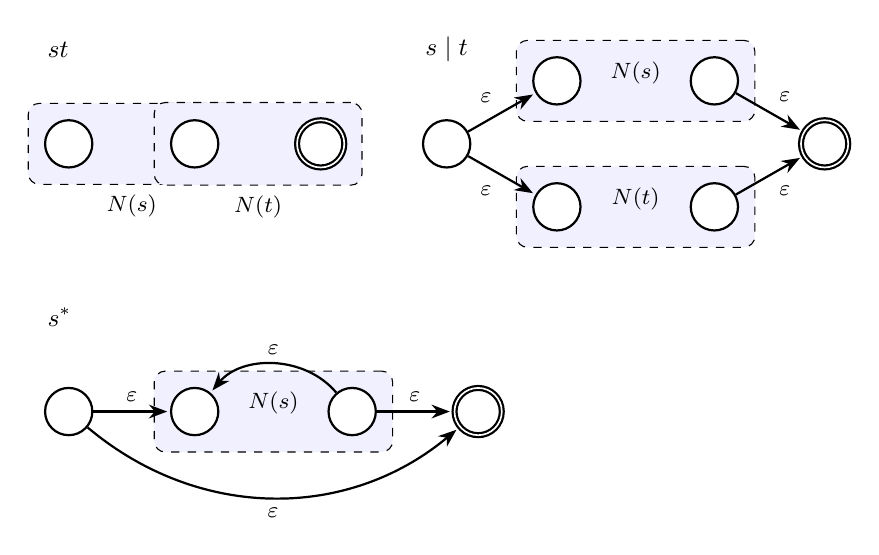
\begin{tikzpicture}[shorten >=1pt, >={Stealth}, thick, every state/.style={minimum size=6mm, inner sep=0pt, fill=white},
    frag/.style={draw, dashed, rounded corners, fill=blue!6, inner sep=2mm, font=\footnotesize}, every edge/.style={draw, ->}, eps/.style={font=\footnotesize}]
  % Concatenation: the accepting state of N(s) becomes the start of N(t).
  \node[font=\small, anchor=west] at (-0.4,1.2) {$st$};
  \node[state] (a) at (0,0) {}; \node[state] (b) at (1.6,0) {}; \node[state, accepting] (c) at (3.2,0) {};

  % Union: a new start branches to both fragments and both rejoin a new accept.
  \node[font=\small, anchor=west] at (4.4,1.2) {$s \mid t$};
  \node[state] (u0) at (4.8,0) {}; \node[state, accepting] (u5) at (9.6,0) {};
  \node[state] (s1) at (6.2,0.8) {}; \node[state] (s2) at (8.2,0.8) {};
  \node[state] (t1) at (6.2,-0.8) {}; \node[state] (t2) at (8.2,-0.8) {};
  \path (u0) edge node[eps, above left] {$\varepsilon$} (s1) (u0) edge node[eps, below left] {$\varepsilon$} (t1)
        (s2) edge node[eps, above right] {$\varepsilon$} (u5) (t2) edge node[eps, below right] {$\varepsilon$} (u5);

  % Star: skip N(s) entirely, or run it and loop back.
  \node[font=\small, anchor=west] at (-0.4,-2.2) {$s^{*}$};
  \node[state] (k0) at (0,-3.4) {}; \node[state] (k1) at (1.6,-3.4) {}; \node[state] (k2) at (3.6,-3.4) {}; \node[state, accepting] (k3) at (5.2,-3.4) {};
  \path (k0) edge node[eps, above] {$\varepsilon$} (k1) (k2) edge node[eps, above] {$\varepsilon$} (k3)
        (k2) edge[bend right=50] node[eps, above] {$\varepsilon$} (k1) (k0) edge[bend right=40] node[eps, below] {$\varepsilon$} (k3);

  \begin{scope}[on background layer]
    \node[frag, fit=(a)(b), label={[font=\footnotesize]below:$N(s)$}] {};
    \node[frag, fit=(b)(c), label={[font=\footnotesize]below:$N(t)$}] {};
    \node[frag, fit=(s1)(s2)] {$N(s)$};
    \node[frag, fit=(t1)(t2)] {$N(t)$};
    \node[frag, fit=(k1)(k2)] {$N(s)$};
  \end{scope}
\end{tikzpicture}
